% Inspired by pgfmanual-en-tikz-arrows.tex coloring and reversed examples.
\usetikzlibrary{arrows.meta}

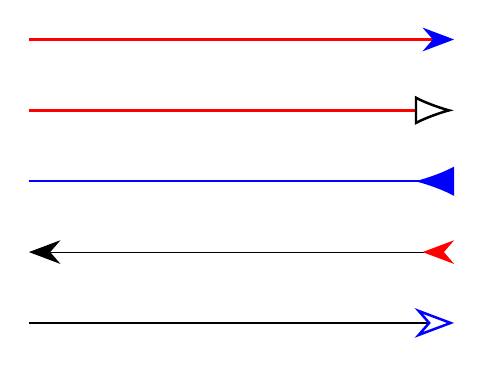
\begin{tikzpicture}[x=1cm,y=1cm]
  \draw[draw=red,line width=0.9pt,-{Stealth[color=blue,length=4mm]}] (0,0) -- (5.4,0);
  \draw[draw=red,line width=0.9pt,-{Latex[color=black,fill=white,length=5mm]}] (0,-0.9) -- (5.4,-0.9);
  \draw[draw=blue,line width=0.9pt,-{Latex[reversed,length=5mm]}] (0,-1.8) -- (5.4,-1.8);
  \draw[{Stealth[length=4mm]}-{Stealth[reversed,length=4mm,color=red]}] (0,-2.7) -- (5.4,-2.7);
  \draw[draw=black,line width=0.9pt,-{Stealth[color=blue,fill=white,length=5mm]}] (0,-3.6) -- (5.4,-3.6);
\end{tikzpicture}
